\documentclass[12pt,titlepage,french]{article}
\usepackage{babel}
\usepackage{graphicx}
\usepackage[margin=2.5cm]{geometry}

\usepackage[hidelinks]{hyperref}
\usepackage{tabularx}
\usepackage{float}
\usepackage[utf8]{inputenc}
\usepackage[T1]{fontenc}
\pagestyle{plain}

\usepackage{booktabs,makecell,tabu}
\usepackage{comment}
\renewcommand\theadfont{\bfseries}

\linespread{1.5}

\newcounter{firstbib}

\begin{document}
%\renewcommand{\thesection}{\arabic{section}} % utilisé pour spécifier la numérotation des sections

\begin{titlepage}
\newcommand{\HRule}{\rule{\linewidth}{0.5mm}}
\center

  
\includegraphics[width=0.45\textwidth]{../../ressources/img_logos/logo_polytech.png}\\[1cm]

  
\includegraphics[width=0.45\textwidth]{../../ressources/img_logos/logo_taglabs.png}


\HRule \\[0.4cm]
{ \huge \bfseries Rapport itération 4\\[0.15cm] }
Classification colorimétrique de nuages de points 3D\\
Version 1.0\\
Le \today \\
\HRule \\[1.5cm]
Ronan Collier,
Mathieu Letrone,
Tri-Thien Truong
\\[1cm]
\end{titlepage}

\tableofcontents % table des matières
\newpage
\listoffigures  % table des figures
\newpage

\section{Rappel des objectifs de l'itération}
Suite à l'itération où nous avions amélioré notre solution, nous avons voulu élargir nos types de filtrages, en utilisant d'autres espaces colorimétriques. De plus, nous avions encore des tâches en cours, que nous devions avancer/finaliser.

Les tâches que nous nous sommes fixées sont les suivantes :

\begin{itemize}
  \item Intégration de fausses couleurs
  \item Revoir la marge d'erreur du filtrage RGB
  \item Terminer la nouvelle méthode de segmentation
  \item Toon mapping \newline
\end{itemize}

\section{Production / réalisation durant l'itération}

Nous développerons ici chaque objectif que nous nous sommes fixé pour cette itération.

\subsection{Intégration de fausses couleurs}

Lors de l'élaboration du cahier des charges avec le client, une des tâches qui nous a été confiée était l'élaboration de fausses couleurs dans un nuage de points en intensité de gris. \newline

Après la première itération, nous avons fait le choix de réaliser notre projet avec un plugin sur le logiciel CloudCompare. Nous n'avions pas pris en compte le fait que le logiciel avait déjà un système de fausses couleurs intégré. \newline

Cette tâche n'est donc plus d'actualité par rapport à ces choix d'implémentation. Nous avons donc décidé de remplacer cette tâche par une nouvelle, qui consiste à l'élaboration d'un nouveau type de filtrage, en utilisant l'espace colorimétrique HSV (Hue - Saturation - Value).

\subsection{Filtrage HSV}

Nous avons pu faire face aux limites du filtrage RGB, où il est difficile d'établir des bornes de couleurs en utilisant uniquement les trois composantes de Rouge, Vert et Bleu. \newline

\begin{figure}[H]
 \caption{\label{} Principe HSV}
 \begin{center}
 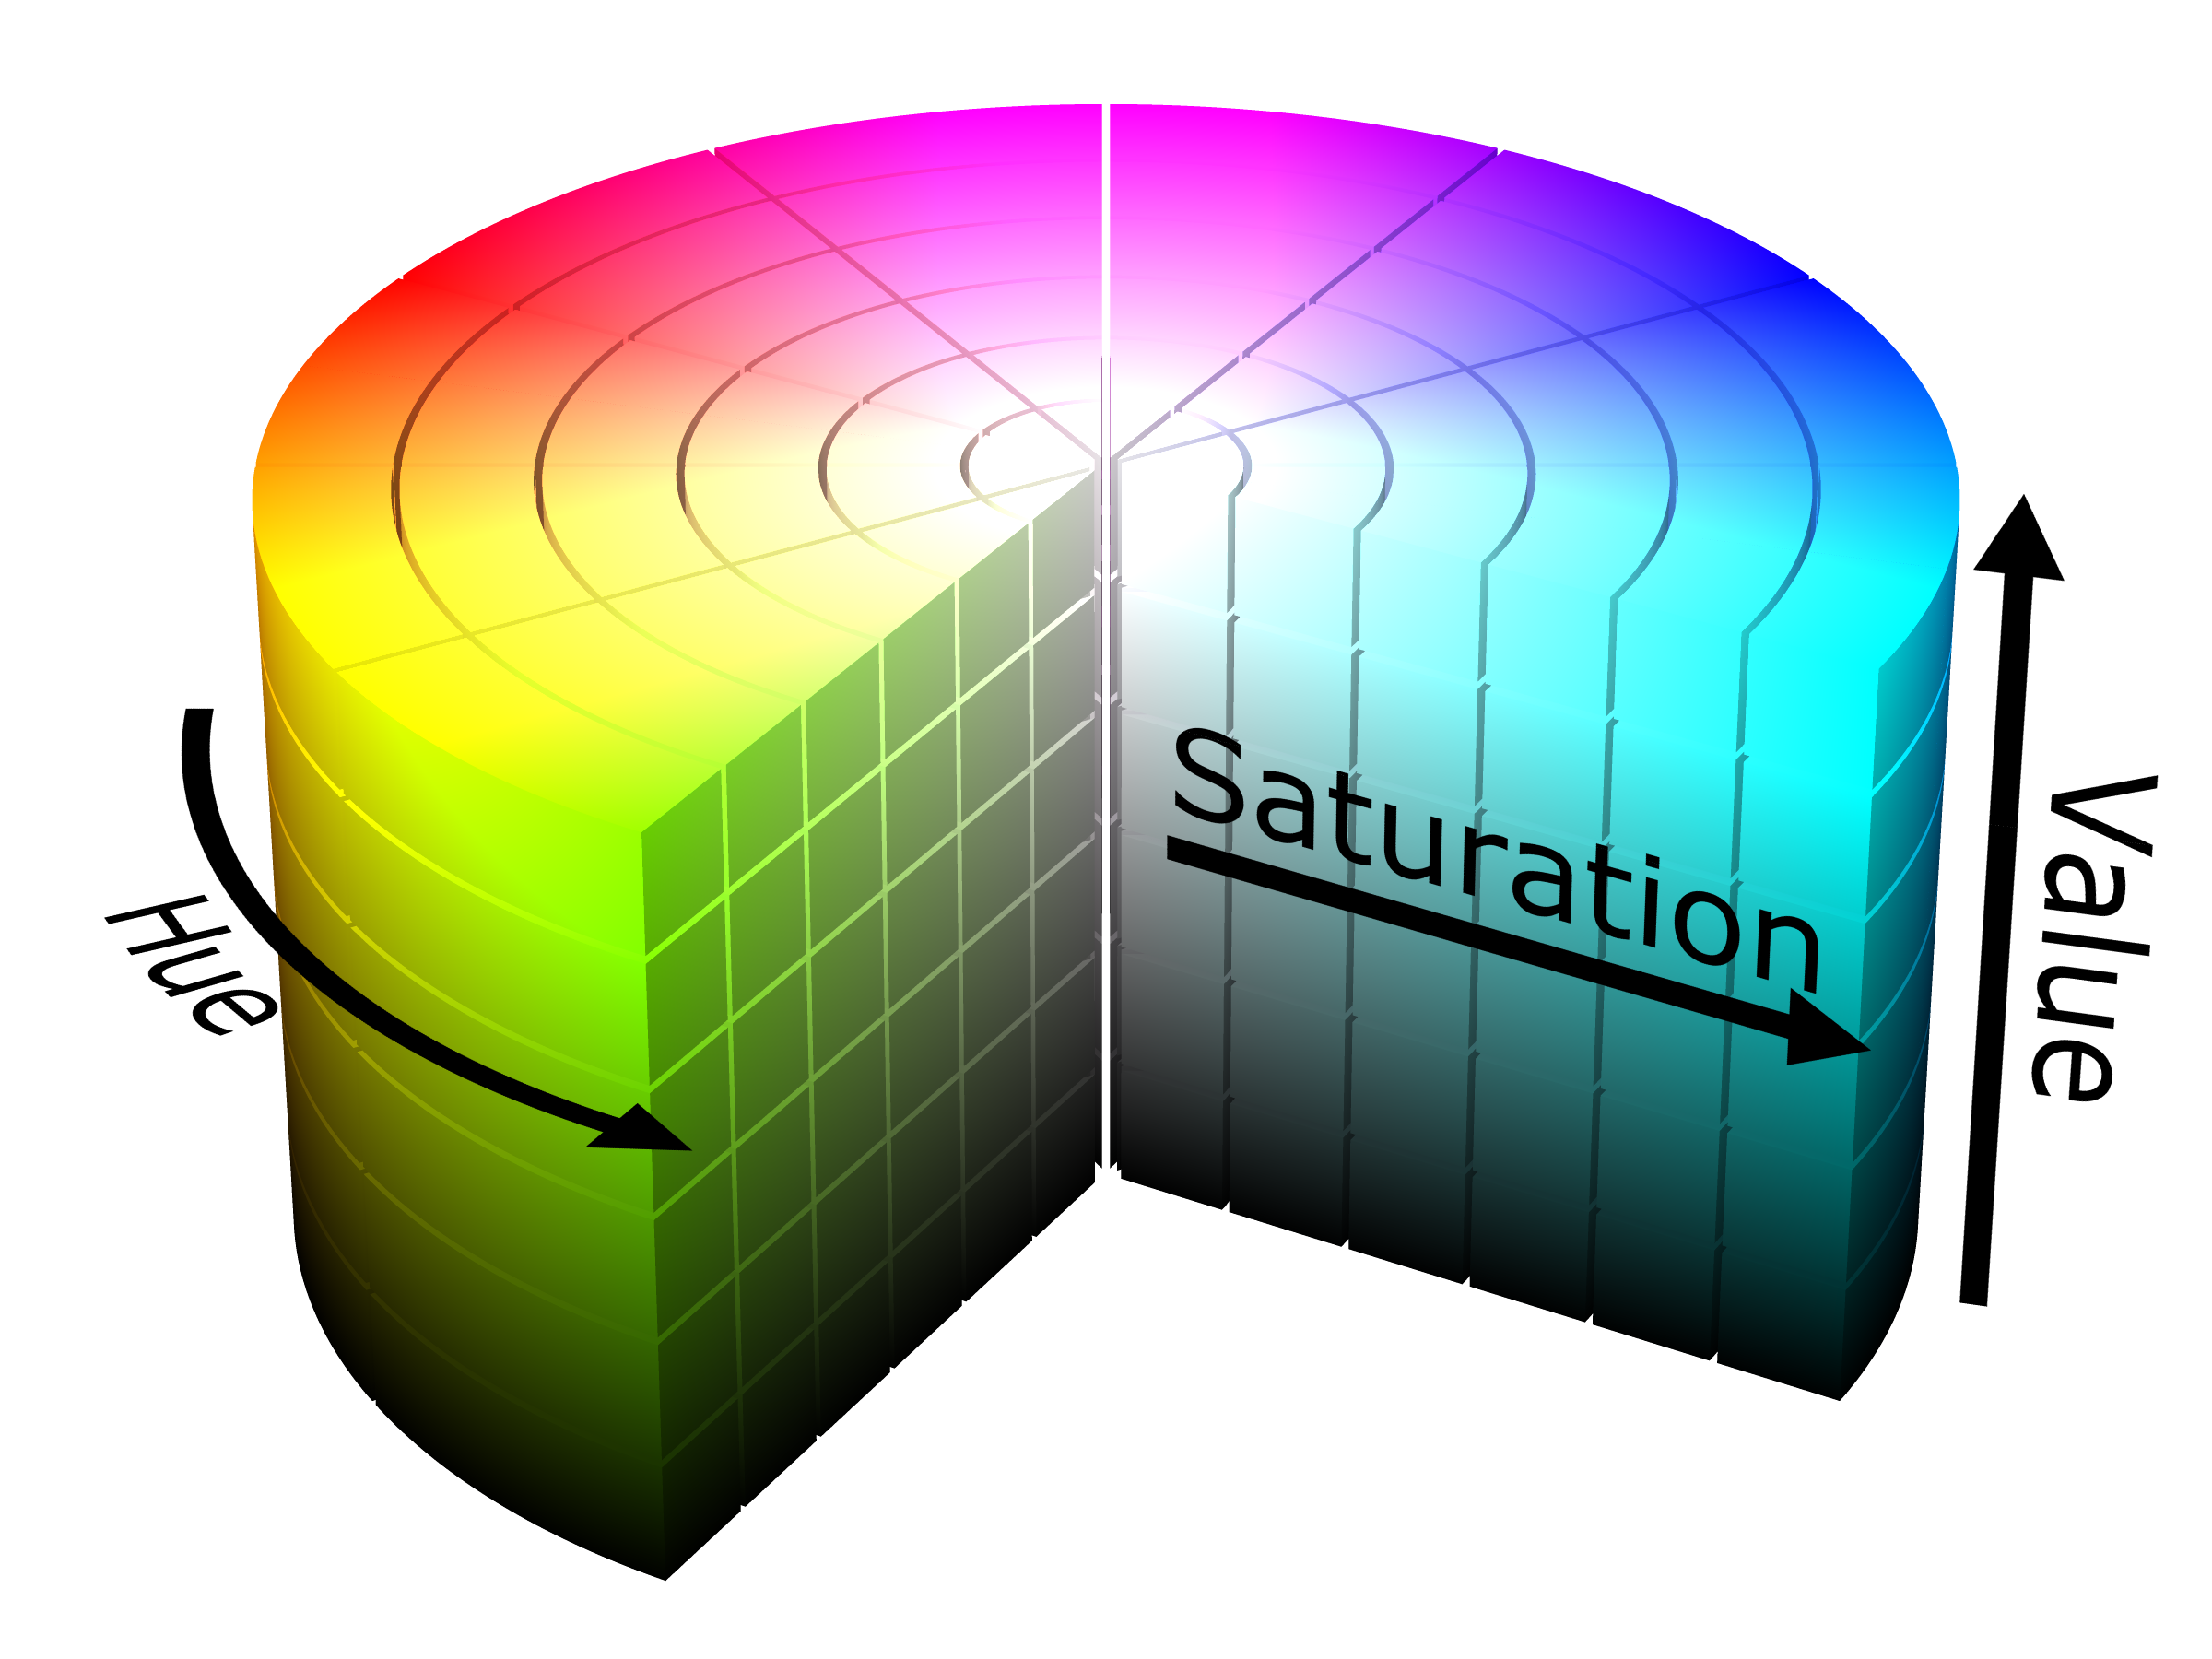
\includegraphics[width=0.75\textwidth]{./img/HSV.PNG}
  \end{center}
\end{figure}

L'espace colorimétrique HSV nous offre un autre moyen de définir les couleurs.  La teinte (Hue) va nous permettre de définir la couleur du point, entre 0 et 360 degrés. La saturation et la valeur, en pourcentage, nous donnent respectivement des informations sur la pureté de la couleur (0 est égal à pas de couleur, donc en nuance de gris entre le blanc et le noir, et 100 pour une couleur vive), et l'intensité lumineuse (0 pour du noir, 100 pour une couleur très claire). \newline

Afin d'obtenir ces valeurs, il nous fallait convertir les valeurs RGB, en HSV. L'algorithme de conversion est disponible sur de nombreux sites internet. Un exemple de l'explication est disponible \cite{B01} ici. \newline

Une fois ceci fait, il nous était alors possible de faire notre interface pour l'utilisateur, afin d'utiliser ce nouveau type de filtrage.

\begin{figure}[H]
 \caption{\label{} Interface filtrage HSV}
 \begin{center}
 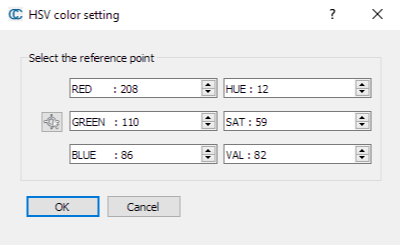
\includegraphics[width=0.75\textwidth]{./img/ui_hsv.PNG}
  \end{center}
\end{figure}

Nous pouvons donc utiliser le point picking pour sélectionner un point dont nous voulons garder dans le filtrage, puis les champs RGB et HSV se remplissent automatiquement. \newline

Au niveau de l'algorithme, nous avons essayé de définir des plages manuellement, en jouant avec nos nouvelles valeurs. Il est plus simple par rapport au RGB, puisque c'est surtout la teinte qui va nous définir la couleur. Il nous reste donc à définir les points qui sont très sombres (et les considérer comme en noir), et inversement très clairs (en blancs). \newline

Pour la définition de nos plages de couleurs, nous nous sommes basé sur le cercle de la teinte des couleurs en 360 degrés, et nous avons définis des seuils pour la saturation et valeur. Nous avons utilisé le site \href{http://colorizer.org}{colorizer.org} \newline

\begin{figure}[H]
 \caption{\label{} Première composante analysée : Saturation - seuil gris}
 \begin{center}
 \makebox[\textwidth][c]{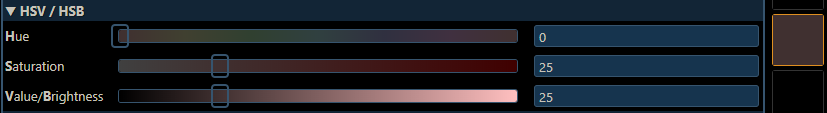
\includegraphics[width=1.2\textwidth]{./img/hsv_color_1.PNG}}
  \end{center}
\end{figure}

Nous avons défini que lorsque la saturation était de 25\% ou en dessous, le point était considéré comme gris, donc la teinte n'influait pas sur la couleur du point. Il est possible de voir la prévisualisation dans la barre "Hue". \newline

La dernière composante Value, est celle qui impacte le plus la couleur du point, entre le noir et le blanc. Avec les prévisualisations, nous avons donc définis que la couleur noir était entre 0 et 25\%, le gris de 26\% à 60\%, et le blanc de 61\% à 100\%. 

\begin{figure}[H]
 \caption{\label{} Première composante analysée : Saturation - test de la valeur}
 \begin{center}
 \makebox[\textwidth][c]{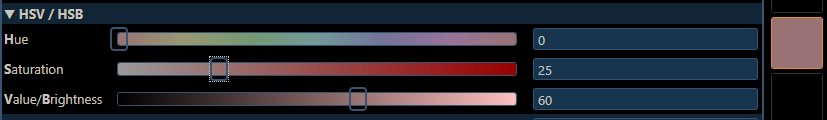
\includegraphics[width=1.2\textwidth]{./img/hsv_color_2.PNG}}
  \end{center}
\end{figure}

Nous pouvons remarquer le fait qu'en modifiant la teinte, ce n'est pas forcément du gris parfait (on peut remarquer la différence de teinte). Néanmoins, il nous fallait quand même définir des valeurs permettant de faire la différence entre les principales gammes de couleurs, sans être trop strict (sinon, la filtrage ne serait pas assez efficace car trop peu de points seraient affichés). \newline

\begin{figure}[H]
 \caption{\label{} Deuxième composante analysée : Valeur - seuil noir}
 \begin{center}
 \makebox[\textwidth][c]{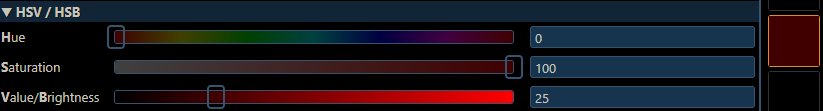
\includegraphics[width=1.2\textwidth]{./img/hsv_color_3.PNG}}
  \end{center}
\end{figure}

Ensuite, lorsque la saturation est au-dessus de 25\%, nous considérons qu'il sera possible de regarder la composante de la teinte, après avoir regardé la valeur. Au niveau de cette dernière composante, si la valeur est entre 0 et 25\%, nous considérons que c'est un point de couleur noir, sinon c'est un point où nous pouvons regarder la teinte.

\begin{figure}[H]
 \caption{\label{} Troisième composante analysée : Teinte - prévisualisation}
 \begin{center}
 \makebox[\textwidth][c]{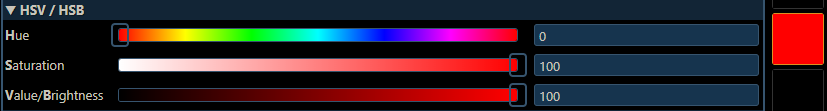
\includegraphics[width=1.2\textwidth]{./img/hsv_color_4.PNG}}
  \end{center}
\end{figure}

Comme nous pouvons le voir, en mettant la saturation à 100\% et la valeur à 100\% (afin d'avoir des couleurs très vives et rapidement voir la différence entre les couleurs), nous pouvons maintenant nous concentrer sur la définition des plages de couleurs. Pour cela, nous nous sommes basés sur la roue représentant les couleurs en 360 degrés.

\begin{figure}[H]
 \caption{\label{} Roue des couleurs}
 \begin{center}
 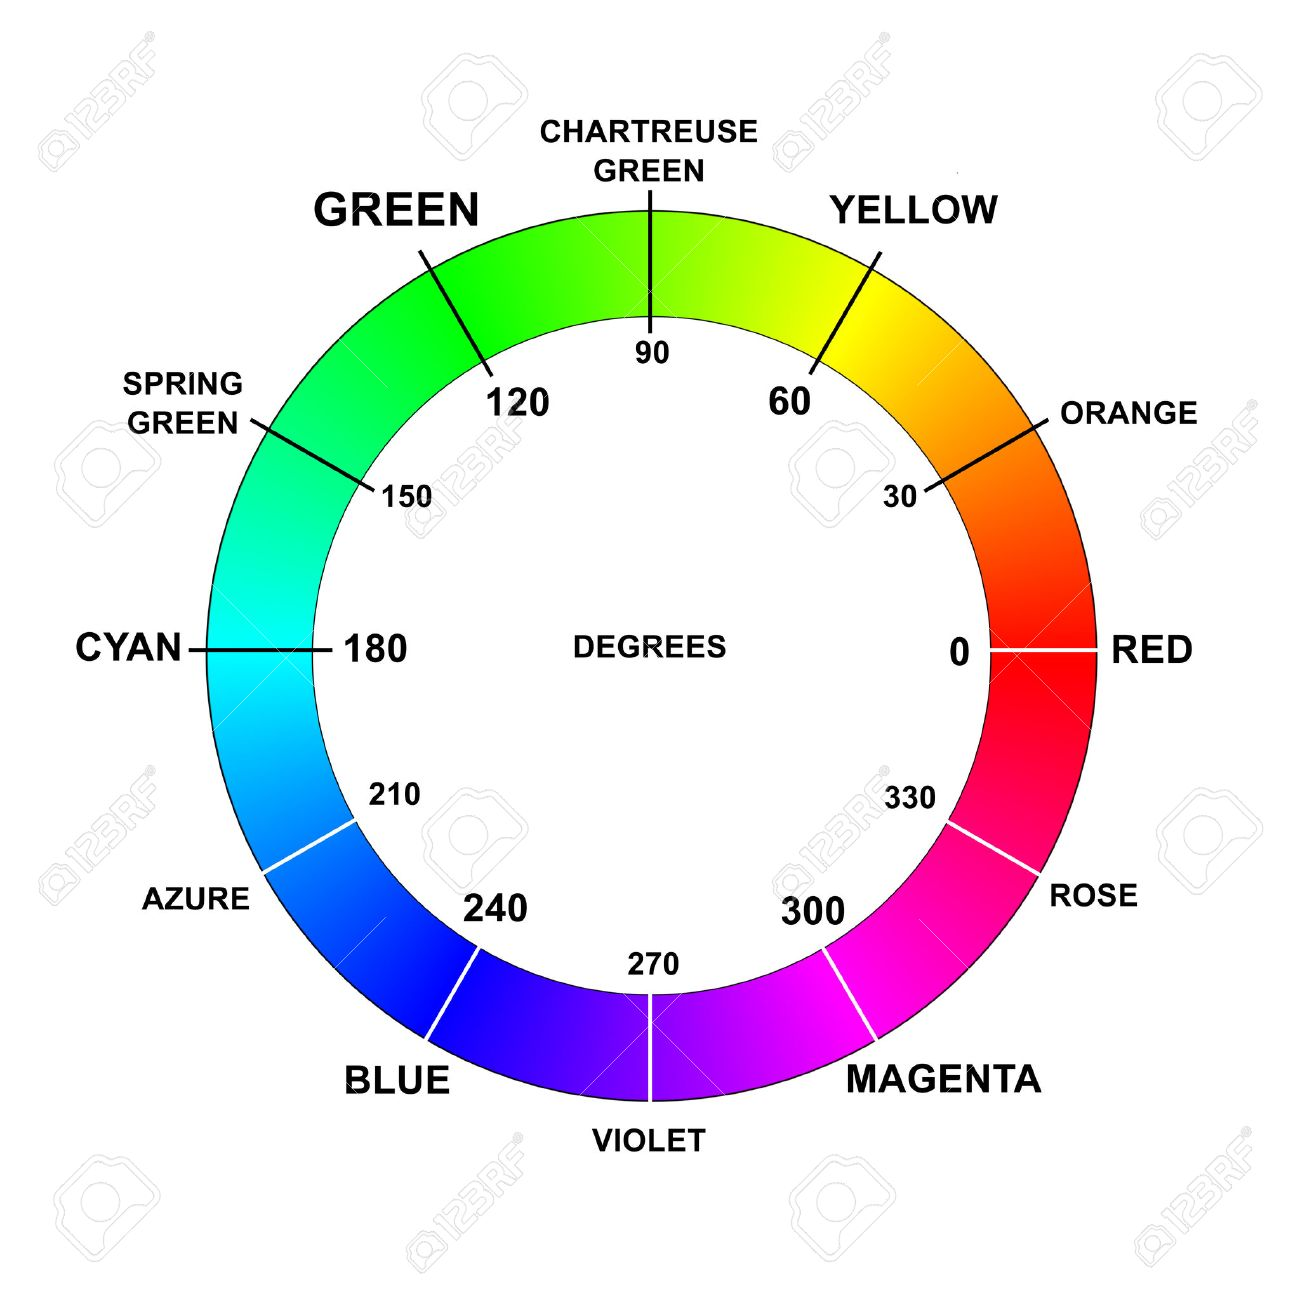
\includegraphics[width=0.7\textwidth]{./img/roue.jpg}
  \end{center}
\end{figure}

Grâce à cette roue, nous avons pu donc définir nos plages pour séparer les principales couleurs. Les plages sont les suivantes :

\begin{itemize}
  \item 0 <= x <= 30 et 330 <= x <= 360 : Rouge
  \item 30 < x <= 90 : Jaune
  \item 90 < x <= 150 : Vert
  \item 150 < x <= 210 : Cyan
  \item 210 < x <= 270 : Bleu
  \item 270 < x <= 330 : Magenta \newline
\end{itemize}

Il nous suffit ensuite de comparer les valeurs dans les champs de l'interface, et de les comparer avec chacun des points du nuage. \newline

Des tests de rapidité n'ont pas encore été effectués, mais le temps est largement acceptable même pour des nuages de points très conséquents.

\begin{figure}[H]
 \caption{\label{} Exemple application filtrage HSV - avant}
 \begin{center}
 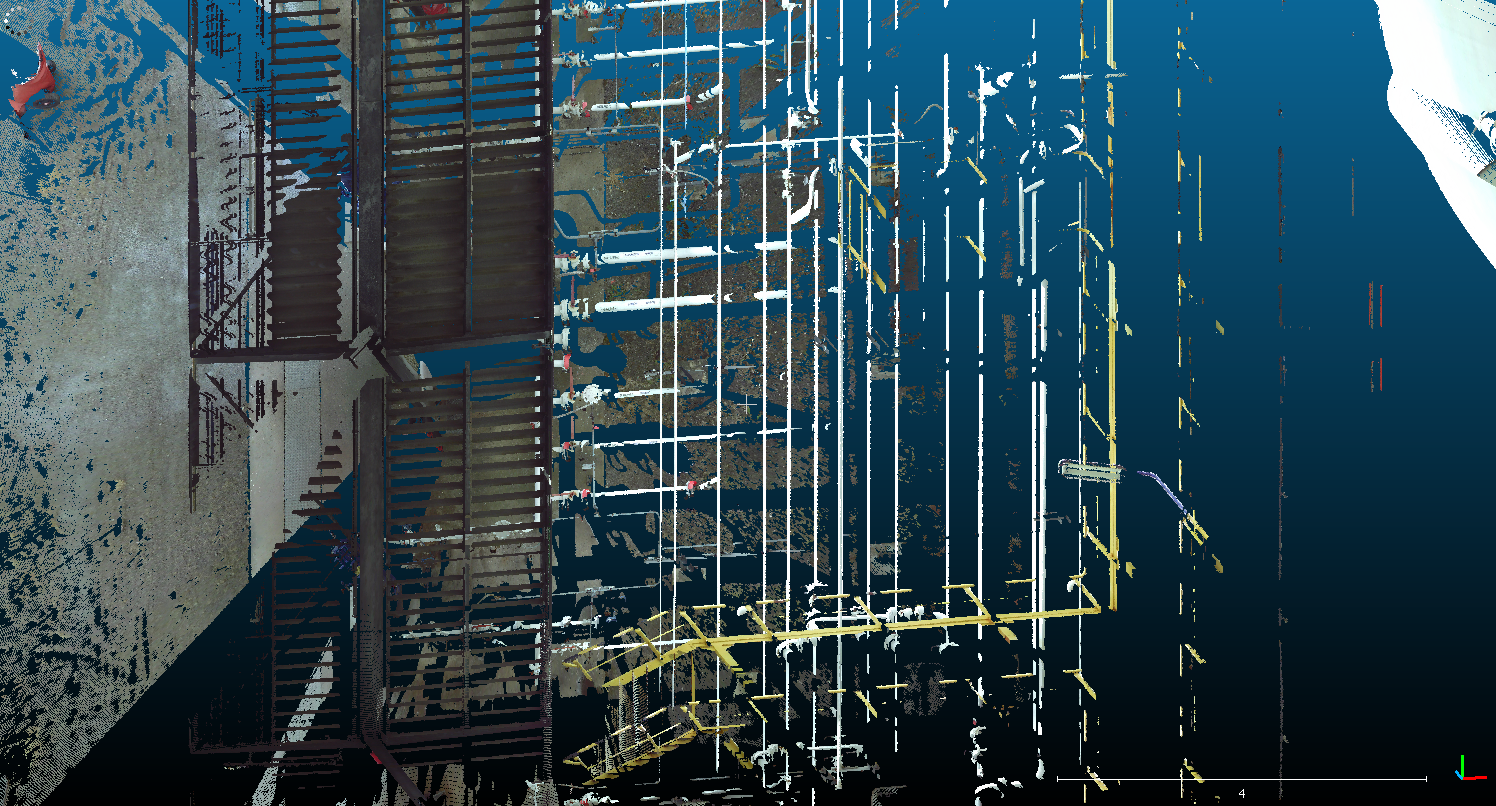
\includegraphics[width=0.8\textwidth]{./img/hsv_before.PNG}
  \end{center}
\end{figure}

\begin{figure}[H]
 \caption{\label{} Exemple application filtrage HSV - après}
 \begin{center}
 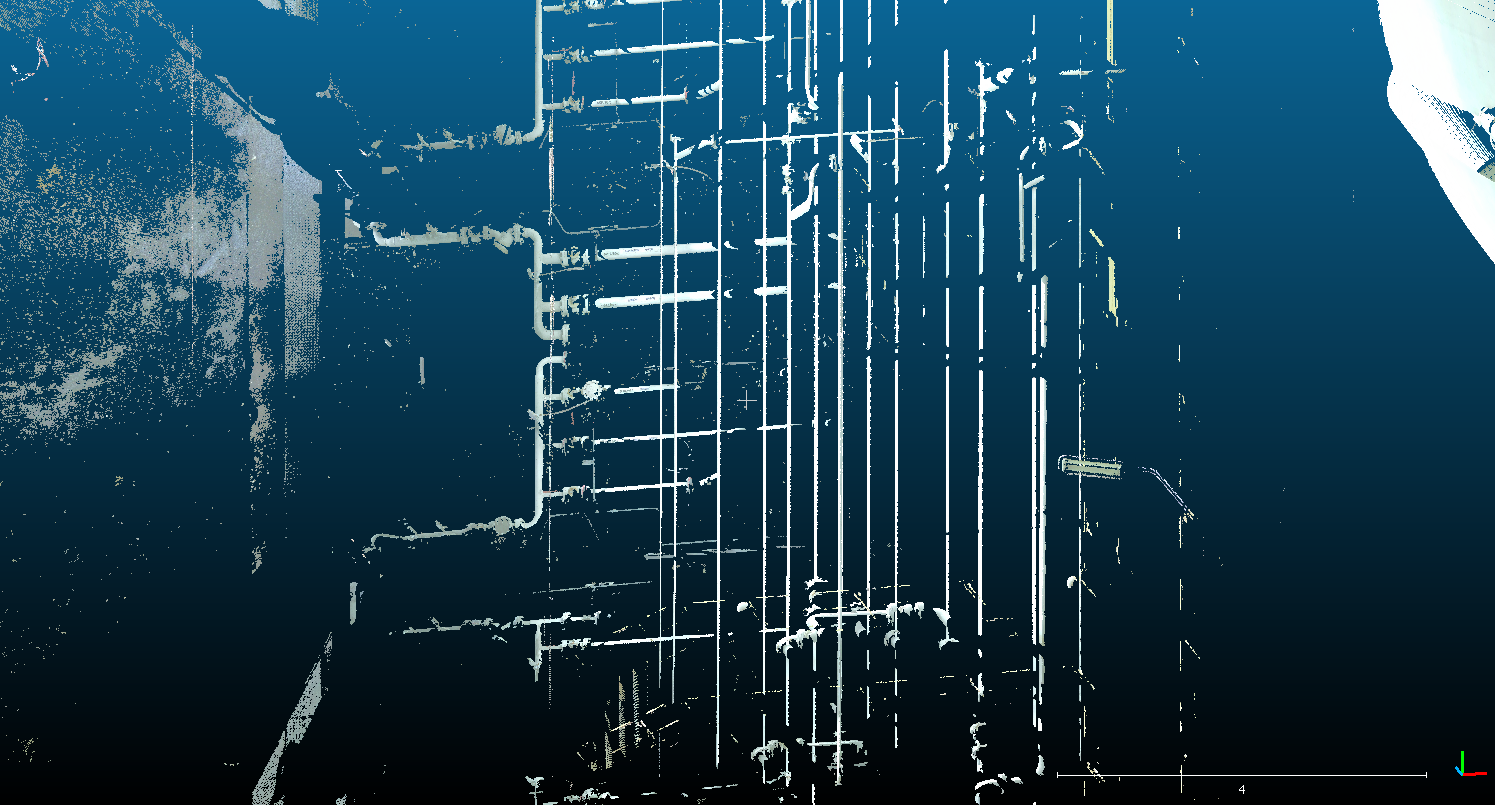
\includegraphics[width=0.8\textwidth]{./img/hsv_after.PNG}
  \end{center}
\end{figure}

Temps d'exécution pour ce nuage (plus de 2 millions de points) : 800 milisecondes.

\subsection{Revoir la marge d'erreur du filtrage RGB}

Suite aux retours du client, nous avons revu le filtrage RGB. En effet, nous avons ajouté un deuxième point à sélectionner, afin de définir les bornes des points à filtrer.

\begin{figure}[H]
 \caption{\label{} Interface filtre RGB}
 \begin{center}
 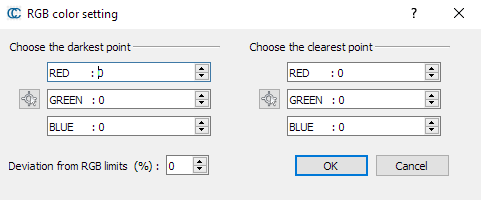
\includegraphics[width=0.9\textwidth]{./img/ui_filter_rgb.PNG}
  \end{center}
\end{figure}

Dans le point à sélectionner dans la partie gauche, il faut prendre le point le plus sombre, qui servira de borne inférieure. Les valeurs devront donc être inférieures aux valeurs de la partie droite. Il est également possible d'ajouter une marge pour agrandir les bornes, afin de réduire l'erreur de l'utilisateur lorsqu'il choisira ses points, et d'obtenir de meilleurs résultats.

\subsection{Terminer la nouvelle méthode de segmentation}

Un algorithme de segmentation était prévu pour être achevé à l'itération précédente. Cependant, des problèmes techniques ne nous ont pas permit d'en arriver à bout. Nous avons donc poursuivit son implémentation. Cet algorithme est séparé en deux étapes. Une première consistant à parcourir le nuage de point afin de créer des régions de couleurs similaires, et une seconde étape dite de "raffinement" afin de réunir les régions similaires. \newline

Ainsi, pour chaque point, on regarde ses voisins en ne gardant que ses voisins les plus proches (en terme colorimétrique) afin de former une région. L'algorithme complet est décrit dans une publication de l'université de \cite{B03} Whuan. \newline

L'algorithme est à l'heure actuelle pratiquement implémenté. Cependant, des erreurs de gestion de la mémoire sont encore présentes, ce qui empêche le plugin de démarrer correctement. La prochaine itération donnera lieu à une correction de cette erreur et à une phase de test de l'algorithme.

\subsection{Toon mapping}

Lors du sprint review de l'itération précédente, le client offrit la suggestion d'apporter une plus-value dans notre solution.
L'implémentation d'un process de "Toon mapping", ce processus a pour but de restreindre le nombre de variations de couleurs au sein du nuage de points. \newline

Ainsi, le nuage apparaîtrait de manière "cartoonesque", cela permettrait de mieux visualiser les éléments par leur couleur et pallier les variations d'intensité d'un même élément.
Ce besoin formulé dans l'itération 3, n'avait pas été prévu ni étudié en amont. Il a donc fallu réaliser des recherches sur ce domaine. \newline

Il y a très peu de documentation sur le toon mapping appliqué sur les nuages de points en 3D. Il a donc fallu faire des recherches sur des méthodes analogues dans le domaine de l'image. 
Dans l'imagerie couleur ou en nuance de gris, il existe différentes méthodes de quantification qui correspondent au principe du "toon mapping". \newline

\begin{itemize}
    \item Octree : partition en arbre avec des branches regroupées ou abandonnées.
    \item Median-Cute : partition en "boîtes".
    \item K-moyennes local : se basant sur k-mean.
    \item Segmentation de l'histogramme.
\end{itemize}

Octree n'a pas été retenu, car il demande beaucoup de mémoire et ça complexité augmente considérablement en fonction de la taille de l'image (d'autant plus que les "petits" scans comptent plus d'un millions de points). Celui des k-moyenne nécessite énormément d'itérations et sa complexité fait partie des NP problème.

Ainsi, pour une première implémentation, nous avons décidé de réaliser un algorithme "simple" celui de segmentation de l'histogramme. Le fonctionnement de cet algorithme est le suivant :
\begin{itemize}
    \item On scinde l'histogramme en autant de groupes qu'on souhaite par composante
    
    (dans le cas du RGB, si on veut 3 sous-groupes par composante, on obtient 27 sous-espaces au sein de l'espace)
    \item On affecte chaque point du nuage à son cluster
    \item Pour chaque cluster, on calcule sa couleur moyenne
    \item Et on affecte cette couleur à tous les points du cluster
\end{itemize}

Actuellement, l'implémentation est terminé, mais la solution est en phase de débuggage pour quelle soit totalement opérationnelle.

\section{Risques éliminés durant l'itération}
Cette itération nous a permis de comprendre encore un peu plus en profondeur le fonctionnement de l'API de CloudCompare.
Cela nous permettra d'éviter de nombreuses erreurs durant le développement.

\section{Feedback}

La soutenance du rapport de description a été pour nous l'occasion d'offrir une vue globale de notre projet au client et au tuteur.
Nous n'avons cependant pas eu l'occasion de réaliser d'autres réunions pour parler en particulier de l'itération. Nous n'avons donc pas de retours sur nos réalisation de l'itération.

\section{Commentaires sur l'itération}

Cette section va présenter nos ressentis sur notre itération. Cela peut correspondre à la façon dont nous avons pu gérer la charge de travail que nous avions prévu en début d'itération, des potentiels imprévus, points positifs/négatifs, et autres.

\subsection{Commentaires sur l'itération de façon générale}

L'itération a grandement été marquée par la rédaction du rapport de description, précisant le travail effectué sur le projet. Son objectif est de détailler le plus clairement possible la solution technique que nous avons apporté, afin que celle-ci puisse être améliorée et maintenue dans le cadre d'un futur projet transversal.
La rédaction de ce rapport a pris beaucoup de temps, laissant moins de créneaux horaire au développement des fonctionnalités prévues dans l'itération.
Notre objectif était de mettre en place les améliorations désirées par le client, ce que nous avons fait.

\subsection{Commentaires sur les méthodes de travail/changements de méthode}

Nous nous sommes moins fixés sur les objectifs que nous avions prévus initialement, mais plutôt sur les demandes client lors des différentes réunions.
La vision du projet sur le long terme semble difficile compte tenu de la situation à la rédaction de ce présent rapport. En effet, la fermeture de Polytech annonce une impossibilité de réaliser des réunions.
Il faudra donc s'axer sur des moyens de communication numériques.
\section{Objectifs de la prochaine itération}

\begin{itemize}
    \item Restreindre l'utilisateur lors de la saisie du filtrage RGB (borne inférieure et supérieure)
    \item Amélioration des plages du filtrage HSV + test de performance
    \item Résoudre les divers problèmes techniques qui empêchent le fonctionnement de l'algorithme de segmentation
    \item Résoudre problèmes et débuggage du toon mapping
    \item Comparer les performances avec un autre algorithme de toon mapping
\end{itemize}

\section{Résumé}
\subsection{Tâches principales réalisées dans l'itération}

\noindent\begin{tabu} to \textwidth {p{0.18\textwidth}X[c2]X[c]X[c4]}\toprule
  \thead{Tâche}&\thead{Responsable}&\thead{Statut}&\thead{Commentaire}\\\toprule
Implémentation filtrage HSV
& Tri-Thien
& Achevé
& Filtrage fonctionnel, améliorable\\\midrule
Revoir la marge d'erreur du filtrage RGB
& Tri-Thien
& Achevé
& \\\midrule
Terminer nouvelle méthode de segmentation
& Ronan
& En cours
& Résoudre le problème de gestion de mémoire + faire des tests \\\midrule
Toon mapping
& Mathieu
& En cours
& Phase de débuggage à faire\\\bottomrule  \\
\end{tabu}

\subsection{Tâches principales à réaliser pour la prochaine itération}

\begin{figure}[H]
 \caption{\label{} Planning itération 5}
 \begin{center}
 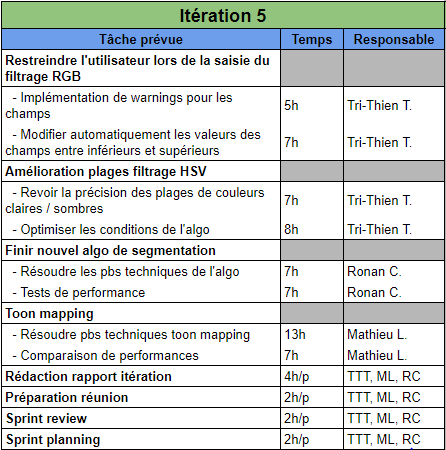
\includegraphics[width=0.8\textwidth]{./img/planning.PNG}
  \end{center}
\end{figure}

\begin{thebibliography}{3}

\bibitem{B01} Conversion RGB - HSV : \newline
\url{https://mattlockyer.github.io/iat455/documents/rgb-hsv.pdf}

\bibitem{B02} Site pour les couleurs : \newline
\url{http://http://colorizer.org}

\bibitem{B03} Qingming Zhan, Yubin Liang, Yinghui Xiao, \textit{Color-based segmentation of point clouds}, 2009

\end{thebibliography}
\end{document}
